\section{How to Use \textit{ThesiX}}
\ThesiX{} have the following structure:

\begin{lstlisting}
\documentclass[a4paper,11pt,openright]{book}
%%-------------------------------------------------------------
\def\iscodiretor{0}
\def\isfamousquote{1}
\def\isdedication{1}
\newcommand{\ThankThesiX}{This document make use of the latex template \textit{ThesiX}, originally made by I. Lombardero and available at https://github.com/ilomdez/ThesiX.}

%%-------------------------------------------------------------
\newcommand{\thesisauthor}{Iv\'{a}n Lombardero Hern\'{a}ndez}
\newcommand{\authordegree}{Graduado en Ciencias F\'{i}sicas}
\newcommand{\university}{UNIVERSIDAD POLIT\'{E}CNICA DE MADRID}
\newcommand{\school}{ESCUELA T\'{E}CNICA SUPERIOR DE INGENIEROS DE TELECOMUNICACI\'{O}N}
\newcommand{\departament}{Departamento de Electrónica Física, Ingeniería Eléctrica y Física Aplicada}
\newcommand{\institute}{INSTITUTO DE ENERG\'{I}A SOLAR}
\newcommand{\thetitle}{ThesiX: latex template for high-quality document formatting with special emphasis on thesis manuscripts - V1.0}
\newcommand{\publicationyear}{\the\year}
\newcommand{\thesisdirector}{Director Name}
\newcommand{\thesisdirectortitle}{Director Degree}
\newcommand{\thesiscodirector}{CoDirector Name}
\newcommand{\thesiscodirectortitle}{CoDirector Degree}

\newcommand{\blankpage}{\clearpage\mbox{}\newpage}
\newcommand{\pdfauthor}{\thesisauthor}
%%-------------------------------------------------------------
\newlength{\currentparskip}
\newenvironment{chapter_resume}% environment name 
{%
  \vspace{1cm}  
  \centering
      
  \setlength{\currentparskip}{\parskip}% save the value
  \begin{minipage}{0.65\textwidth}\setlength{\parindent}{0.5cm}
  \begin{itshape}
}% 
{\end{itshape}\end{minipage}\vspace*{\fill}\newpage}% end code
%-------------------------------------------------------------
\newenvironment{project}[4]{
\begin{itemize}[align=left, leftmargin=10mm, labelsep=1mm, labelwidth=2mm, itemindent=0pt]
	%\setlength{\itemindent}{-0.3in}
 	\item[\textbf{Title:}] #1
 	\item[\textbf{P.I:}] #2
 	\item[\textbf{Funding:}] #3
 	\item[\textbf{Duration:}] #4
\end{itemize} 
}
{\vspace{.5cm}}

%---------------------------------------------------------------
\newlength{\thicktopline}
\setlength{\thicktopline}{0.1em}
\newlength{\thickbottomline}
\setlength{\thickbottomline}{0.1em}
\newlength{\tablerowheight}
\setlength{\tablerowheight}{-1em}
%%
\newcommand{\app}{Appendix}
\newcommand{\aumet}{AuGe/Ni/Au}
\newcommand{\cha}{Chapter}
\newcommand{\equ}{Equation}
\newcommand{\ies}{Solar Energy Institute}
\newcommand{\iiiv}{III\=/V}
\newcommand{\iv}{I\nobreakdash-V}
\newcommand{\InN}{GaInNAs}
\newcommand{\InNSb}{GaInNAsSb}
\newcommand{\fig}{Figure}
\newcommand{\macmsq}{mA/cm\textsuperscript{2}}
\newcommand{\NSb}{GaNAsSb}
\newcommand{\pdmet}{Pd/Ge/Ti/Pd/Al}
\newcommand{\phosphoric}{H\textsubscript{3}PO\textsubscript{4}:H\textsubscript{2}O\textsubscript{2}:H\textsubscript{2}O}
\newcommand{\nip}{\textit{n\=/i\=/p}}
\newcommand{\pn}{\textit{pn}}
\newcommand{\sect}{Section}
\newcommand{\sj}{single\=/junction}
\newcommand{\soa}{state\=/of\=/the\=/art}
\newcommand{\tab}{Table}
\newcommand{\ThesiX}{\textit{ThesiX}}
\newcommand{\TJ}{GaInP/Ga(In)As/Ge}
\newcommand{\unitsscr}{$\Omega$·cm\textsuperscript{2}}
\newcommand{\unitssr}{$\Omega$/$\square$}

\newcommand{\Msup}{\$^\{}
\newcommand{\Msupe}{\}\$}

 
% Packages used in ThesiX
%%-----------------------------------------------------------
% Embebing Fonts
% ¿Automatic in TexMaker? If you are using TeXStudio in Windows, Go to Options-> Configure TeXstudio->Commands->Ps2Pdf. In that field, just paste ps2pdf.exe -dPDFSETTINGS#/prepress -dEmbedAllFonts#true -dMaxSubsetPct#100 -dCompatibilityLevel#1.3 %.ps


%%-----------------------------------------------------------
% Debuging
%\usepackage{showframe}
%\usepackage{blindtext}
%\listfiles


%%------------------------------------------------------------
% Metadata
\usepackage[pdftex,hidelinks]{hyperref}
\hypersetup{pdftitle=\thetitle{}, pdfauthor={\thesisauthor}}
\hypersetup{pdfsubject={ThesiX LaTeX Template}}
\hypersetup{pdfkeywords={LaTeX, Thesis, Template, ILH}}


%%-----------------------------------------------------------
% General packages about encoding and appeareance
\usepackage[utf8]{inputenc}
\usepackage[top=1.75cm,bottom=1.75cm,left=2.5cm,right=2.5cm,includeheadfoot,asymmetric]{geometry}
\usepackage{newunicodechar}
\newunicodechar{µ}{\ensuremath{\mu}}
\newunicodechar{°}{º}
%\newunicodechar{α}{\ensuremath{\alpha}} %Esto se puede utilizar para caracteres chungos si va mal junto con el newunicodechar - fontec y inputtec de arriba , para los % quizas--
\usepackage{eurosym}
\usepackage{indentfirst}
\usepackage{enumitem}
\usepackage{amsmath}
\usepackage{amssymb} %Careful with the font loaded!! If it has already loaded the symmbols it may stop working
\usepackage{multirow}
%\usepackage{multicol}
\usepackage[shortcuts]{extdash} % unbreakable hyphen - dash
%\usepackage{xparse} %newcommand and newenvironment with multiple optional arguments
\usepackage{verbatim}
\usepackage{listings}
\lstset{
  basicstyle=\ttfamily,
  columns=fullflexible,
  frame=single,
  breaklines=true
}
\usepackage{pdfpages}


%%------------------------------------------------------------
% Titles, chapters, headers, etc.
\usepackage{fancyhdr}
\usepackage{titlesec}
\titleformat{name=\chapter,numberless}
	{\filcenter\normalfont\huge\bfseries}{}{20pt}{\Huge}[\vspace{0.0ex}\titlerule]
%
\titleformat{name=\chapter}[display]
	{\Huge\rm\filcenter}
	{\titlerule[2pt]%
	\vspace{-3pt}%
	\titlerule
	\vspace{1pc}%
	\Huge\rm\bfseries\MakeUppercase{\chaptertitlename} \Huge\rm\bfseries\MakeUppercase{\thechapter}}
	{1pc}
	{\titlerule
	\vspace{1pc}%
	\Huge}
%
\titleformat*{\subsubsection}{\large\itshape} % Definition of subsubsection style
\setcounter{secnumdepth}{3} % Depth of sections numbering - 3 =subsubsections
\setcounter{tocdepth}{2} %Depth of table of content - 2 =subsections


%%------------------------------------------------------------
% REFERENCES & GLOSSARIES
\usepackage{bookmark} % allows to set bookmarks manually, useful for abstract etc
\usepackage{cleveref} % for subfigures references and more
\usepackage{nameref}  % to reference section names
\newcommand{\itnameref}[1]{\textit{\nameref{#1}}} % reference section name in italics
\newcommand{\quitnameref}[1]{``\textit{\nameref{#1}}''} % reference section name in italics and quotation mars
\usepackage{tocbibind}
\usepackage[toc, acronym, nopostdot, section=chapter, automake=immediate]{glossaries}  %sort=def hace que super no pueda separar por grupos de palabras
% sanitizesort=false hace que pase del \textit{•} y cosas de esas y organice directamente por lo que ve dentro aunque según he leido ralentiza bastante - guia page 15
\makeglossaries
\usepackage[style=alphabetic, backend=biber, sortcites=true, sorting=ynt, defernumbers=true, maxbibnames=99]{biblatex}
\addbibresource{./bibliography/ThesisRef.bib}
%\assignrefcontextentries[]{*}
%\usepackage[hyphenbreaks]{breakurl}
%\usepackage{csquotes}
%
\DefineBibliographyStrings{english}{%
  bibliography={References},
}
\defbibheading{secbib}[\bibname]{%
  \section*{#1}%
  \markboth{#1}{#1}
}
%
\defbibenvironment{bibliographyNUM}
  {\list
     {\printtext[labelnumberwidth]{%
        \printfield{prefixnumber}%
        \printfield{labelnumber}}}
     {\setlength{\labelwidth}{\labelnumberwidth}%
      \setlength{\leftmargin}{\labelwidth}%
      \setlength{\labelsep}{\biblabelsep}%
      \addtolength{\leftmargin}{\labelsep}%
      \setlength{\itemsep}{\bibitemsep}%
      \setlength{\parsep}{\bibparsep}}%
      \renewcommand*{\makelabel}[1]{\hss##1}}
  {\endlist}
  {\item}


%%------------------------------------------------------------
% IMAGES
\usepackage{float} % Useful for tables as well
\usepackage{graphicx}
\usepackage{caption}
\usepackage{subcaption}
\captionsetup{labelfont=bf,justification=justified,font=footnotesize}
%\usepackage{wrapfig}
\graphicspath{
{./images/}
{./images/Title/}
{./images/Cover/}
{./images/Intro/}
}
\usepackage{svg}
%\setsvg{inkscape={C:/"Program Files"/Inkscape/inkscape.exe -z -D}}
%\usepackage[inkscapeexe=C:/Program~Files/Inkscape/inscape.exe]{svg}
\svgpath{{./images/}{./images/cover/}{./images/chapter1/}{./images/chapter2/}{./images/chapter3/}{./images/chapter4/}{./images/chapter5/}{./images/title/}}
%\def\eattif#1.tif{#1}
%\DeclareGraphicsRule{.tif}{png}{.png}{`convert #1 \eattif#1-tif-converted-to.png }
\usepackage{epstopdf}
\epstopdfDeclareGraphicsRule{.tif}{png}{.png}{convert #1 \OutputFile}
\AppendGraphicsExtensions{.tif}


%%-------------------------------------------------------------
% TABLES
\usepackage{tabularx}
\usepackage{makecell} %group words
\usepackage{booktabs}
\usepackage{array}
\usepackage{arydshln} % dash lines
\renewcommand\tabularxcolumn[1]{m{#1}}% for vertical centering text in X column - Not working always somehow
\newcolumntype{Y}{>{\centering\arraybackslash}X} % same as X but horizontally allinged
\newcolumntype{M}{>{\centering\let\newline\\\arraybackslash\hspace{0pt}}m{.5cm}}
%\newcolumntype{N}[1]{>{\centering\let\newline\\\arraybackslash\hspace{0pt}}Y}
\newcolumntype{n}{>{\centering\arraybackslash}m} % same as m but horizontally allinged
%%------------------------------------------------------------
% Force Words Htphenation
\hyphenation{
Ga-In-N-As-Sb
}
% Acronym definitions
%
% A
\newglossaryentry{abc}{type=\acronymtype, name={ABC}, description={ABC example}}
\newglossaryentry{acronym1}{type=\acronymtype, name={AE1}, description={Acronym example 1}}
\newglossaryentry{acronym2}{type=\acronymtype, name={AE2}, description={Acronym example 2}}
%
% B
\newglossaryentry{b_acronym}{type=\acronymtype, name={BEA}, description={B example of acronym}}
%
% C
\newglossaryentry{c_acronym}{type=\acronymtype, name={CEA}, description={C example of acronym}}
%
%
% D
%
% E
%
% F
%
% G
%
% H
%
% I
%
% J
%
% K
%
% L
%
% M
%
% N
%
% O
%
% P
%
% Q
%
% R
%
% S
%
% T
%
% U
%
% V
%
% W
%
% X
%
% Y
%
% Z
% Symbols definitions
%
% A
\newglossaryentry{symbol1}{name={\textit{S\textsubscript{1}}}, description={Symbol example 1}}
\newglossaryentry{symbol2}{name={\textit{S\textsubscript{2}}}, description={Symbol example 2}}
\newglossaryentry{alpha_int}{name={$\alpha_int$}, description={Intrinsic Absorption coefficient}}
%
% B
\newglossaryentry{b_symbol}{name={B\textsuperscript{5}}, description={B example of symbol}}
%
% C
\newglossaryentry{c_symbol}{name={C\textsubscript{t}}, description={C example of symbol}}
%
%
% D
%
% E
%
% F
%
% G
%
% H
%
% I
%
% J
%
% K
%
% L
%
% M
%
% N
%
% O
%
% P
%
% Q
%
% R
%
% S
%
% T
%
% U
%
% V
%
% W
%
% X
%
% Y
%
% Z
%-------------------------------------------------------
\begin{document}
\pagenumbering{gobble}
\begin{titlepage}
   \begin{center}
   		%\fontsize{17}{17}
   		%\selectfont
		\begin{LARGE}
		\textbf{\university}
		\end{LARGE}		   		
   		 		
   		\vspace*{2.5cm}
		
		\begin{normalsize}
		\school
 		\end{normalsize}
 		
 		\vspace*{1cm}
 		
 		
\includegraphics[scale=0.45]{LOGO_ESCUELA.pdf}

		\vspace{4.5cm}
		\vspace{\fill}

		\begin{Huge}
		\thetitle
		\end{Huge}
		
		\vspace{2.5cm}
		
		\begin{LARGE}
		\textbf{TESIS DOCTORAL} 
		\end{LARGE}
		
		
		\vspace{3cm}
		
		\begin{LARGE}
		\thesisauthor
		\end{LARGE}
		
		\begin{Large}
		\authordegree
		\end{Large}
		
		\vspace{1cm}
			
		\begin{LARGE}
		\publicationyear
		\end{LARGE}
   \end{center}
\end{titlepage}
\begin{titlepage}
   \begin{center}
   		%\fontsize{16}{16}\selectfont\textbf{\universidadupper}
		%\fontsize{16}{16}\selectfont
		\begin{LARGE}
		\textbf{\institute}
		\end{LARGE}
		
 		\begin{normalsize}
 		\departament
 		\end{normalsize}
		
		\vspace*{2.5cm}
		
		\begin{normalsize}
		\school
 		\end{normalsize}
% 		\begin{small}
%		\escuelaupper
% 		\end{small}		
		\vspace*{0.5cm}
 		
 		
\includegraphics[scale=0.4]{LOGO_ESCUELA.pdf}
		
		\vspace*{\fill}
		
		\begin{Huge}
		\thetitle
		\end{Huge}

		
		\vspace{2.5cm}
		
		\begin{table}[h]
		\LARGE
		\centering
		\begin{tabular}{l  l}
		
		\textbf{Autor:} & \thesisauthor \\
		 & \authordegree \\
		 & \\
		\if\iscodiretor0
		\textbf{Director:} & \thesisdirector \\
		\else
		\textbf{Directores:} & \thesisdirector \\
		\fi
		 				   & \thesisdirectortitle \\ 
						   \if\iscodiretor1						   
						   &  \thesiscodirector \\
						   & \thesiscodirectortitle \\
						   \fi
		\end{tabular}
		\label{tab:SecondTitle}
		\end{table}
				
		\vspace{1.5cm}
		
		\begin{LARGE}
		\publicationyear
		\end{LARGE}			
				
   \end{center}
\end{titlepage}
\newpage
\blankpage
\textbf{Tribunal nombrado por el Magfco. Y Excmo. Sr. Rector de la}

\textbf{Universidad Polit\'{e}cnica de Madrid.}

\vspace*{1cm}

PRESIDENTE:

\vspace*{1.5cm}

VOCALES:

%\indent\indent Guido es
%
%\indent\indent un poco retrasado
%
%\indent\indent y mi template es cojonudo
%{\setlength{\parindent}{0cm}
%\begin{table}[h]
%	\begin{tabular}{@{}ll}
%		VOCALES:	& Gerald Siefer \\
%					& Marta Vivar \\
%					& Eduardo Román Medina \\		
%	\end{tabular}
%\end{table}
\vspace*{3cm}

SECRETARIO:

\vspace*{1.5cm}

SUPLENTES:

\vspace*{3.5cm}

\hfill{Realizado el acto de defensa y lectura de la Tesis en Madrid,}

\hfill{el día \underline{\hspace{1cm}} de \underline{\hspace{2.5cm}} de 2019.}

\vspace*{1cm}

Calificaci\'{o}n:

\vspace*{2cm}

EL PRESIDENTE \quad\quad\quad\quad\quad\quad\quad\quad\quad\quad LOS VOCALES

\vspace*{2cm}

EL SECRETARIO
\blankpage
\vspace*{3.5cm}
\begin{flushright}
\textit{Dedication if any}
\end{flushright}
\newpage
\blankpage
\vspace*{3.5cm}
\begin{flushright}
\textit{Famous quote if any.\\Author}
\end{flushright}
\newpage
\blankpage
\pagestyle{fancy}
\fancyhf{}
%\renewcommand{\chaptermark}[1]{\markboth{#1}{}}
%\renewcommand{\sectionmark}[1]{\markright{\thesection\ #1}}
\fancyhead[CEO]{\itshape\nouppercase{\leftmark}}
\fancyfoot[C]{\thepage}
\setlength{\headheight}{15pt}

%\fancyhf{}
%\fancyhead[LE,RO]{\thepage}
%\fancyhead[LO]{\itshape\nouppercase{\rightmark}}
%\fancyhead[RE]{\itshape\nouppercase{\leftmark}}
\chapter*{Acknowledgements} \markboth{Acknowledgements}{}
Acknowledgements if any.
\frontmatter
\pdfbookmark[0]{Resumen}{Resumen}
\chapter*{Resumen} \markboth{Resumen}{}
Resumen means Abstract in Spanish, but obviously it should be replaced by the corresponding word in the mother tongue of the author. In my opinion, this should be always before the Abstract, as probably the acknowledgements will be mostly written in the author's mother tongue. Therefore it make sense to put these two sections together, and leave the Abstract closer to the rest of the document which will be probably written in English. In any case this depends on the personal view of the user.
\pdfbookmark[0]{Abstract}{Abstract}
\chapter*{Abstract} \markboth{Abstract}{}
Thesis abstract.
\tableofcontents
%\addcontentsline{toc}{chapter}{\listfigurename}
\listoffigures
%\addcontentsline{toc}{chapter}{\listtablename}
\listoftables
\setlength{\glsdescwidth}{0.7\textwidth}
\printglossary[type=main, style=super, nonumberlist, title=List of Symbols] %style=super, nogroupskip,
\setlength{\glsdescwidth}{0.8\textwidth}
\printglossary[type=\acronymtype, style=super, nonumberlist, title=List of Acronyms]
\mainmatter
\pagestyle{fancy}
\fancyhf{}
%\renewcommand{\chaptermark}[1]{\markboth{#1}{}}
%\renewcommand{\sectionmark}[1]{\markright{\thesection\ #1}}
%\fancyhead[R]{\textcolor{gray}{Mock Draft}}
\fancyhead[RO]{\rightmark}
\fancyhead[LE]{\leftmark}
\fancyfoot[RO,LE]{\thepage}
\setlength{\headheight}{15pt}
\renewcommand{\sectionmark}[1]{\markright{\thesection.\ #1}}
\renewcommand{\chaptermark}[1]{\markboth{\thechapter.\ #1}{}}
%\renewcommand{\chaptermark}[1]{\markleft{\thechapter.\ #1}}
%\fancyhead[RE]{\fontsize{10}{10}\selectfont\leftmark}
%\renewcommand{•}{•}
\chapter{Introduction}\label{ch:Intro}
\begin{chapter_resume}
This chapter presents the thesis introduction.\\

The current scenario of the photovoltaic market is briefly reviewed, analysing the historical trends and future perspectives of the most important technologies.\\

This leads to the revision of the \soa{} of multijunction solar cells, on which this thesis focuses on. The three main approaches (new compound materials, metamorphic buffers and the wafer bonding technique) are analysed, summarizing their benefits and drawbacks.\\

The aforementioned revision set the basis to establish the thesis goals, which is devoted to enhancing the potential of multijunction solar cells by developing advanced architectures. One of the main pathways has been the traditional approach based on increasing the number of subcells, but other improvements such as the thinning of substrates or the use of graphene as a top contact have also been explored. Accordingly, a detailed explanation of the main objectives to be accomplished is provided.\\

Afterwards, the outline followed in the thesis to illustrate the work carried out is explained to ease the reader task of finding whatever required information.\\

Finally, the framework which has surrounded this thesis is described, accounting for the funding, the means provided by the group, colleagues or third party partners as well as the main achievements attained through this thesis.\\
\end{chapter_resume}

\section{About \textit{ThesiX}}
\ThesiX{} was created during the redaction of my Ph.D. thesis. I found it difficult to find a \LaTeX{} template that eases the template build up while being easily extensible and customizable. Although there are some good works available, all of them fail to provide an out of the box template, easy to understand and modify without strong design constraints. My purpose is that this template will be use as the basis of any other work, modifying this template as necessary. Even if it is design to work as it is, all users are highly encourage to learn at least a basic \LaTeX{} and improve the template.

The latest template release is available at https://github.com/ilomdez/ThesiX for use under license GPL-3.0. It would be highly appreciated if the user thank the template availability explicitly stating in their document so, for instance by the use of the defined command ``\textbackslash{}ThankThesiX'' or with any other sentence that fits better the user while maintaining the same meaning and explicitly staying the repository webpage and the \ThesiX{} author name.:\\

	\ThankThesiX{}\\

\ThesiX{} is its own manual and example, which means that the manual has been built using the \ThesiX{} template. If the files are compiled as downloaded the output file will be this very same manual. Accordingly, several examples of all that can be achieved with \ThesiX{} has been exemplified in the manual, so that every user can easily get examples of how to achieve most usual figures, tables or layouts in a thesis document.

I just would like to finish remembering that this is NOT a \LaTeX{} manual and that every user is encourage to learn at least the basis by themselves. This is easily accomplished given the tremendous amount of information and tutorials available on-line. The \LaTeX{} community has made an incredible effort during the last years so that everyone can learn on their own. In any case, \ThesiX{} is built to be used by non\=/\LaTeX{} users straightforward.

Any requirement or suggestion should be requested at the Github webpage or my LinkedIn personal webpage (https://www.linkedin.com/in/ilomdez/). In any case, \ThesiX{} is an ongoing work which is carried out in my free-time and accordingly, its extension, readability, number of examples or level of detail will be improved when possible. Nevertheless, the \LaTeX{} template is fully functioning and the main remaining work is to finish the manual.
\section{Installation} % Dar más detalles
In order to use \ThesiX{} clone or download the whole repository at https://github.com/ilomdez/ThesiX. Compiling the code should be pretty straight forward, although some steps might vary depending on the operative system and the compiler chosen:

\subsection{Windows - TextMaker - MikTex}
This section has been tested under Windows 10, TexMaker 5.0.3 and MikTex 2.9.6972. The version of each package used in the compilation of the latest \ThesiX{} manual can be found in the log file in the main folder of the repository.

Follow the instructions below:
\begin{enumerate}
	\item Download the corresponding MikTex version (https://miktex.org/download) and install it.
	\item Download the corresponding TexMaker version (https://www.xm1math.net/texmaker/) and install it.
	\item Configure TexMaker as depicted in \fig\,\ref{fig:Intro_TexMakerConf}.

%%%%%%%%%%%%%%%%%%
\begin{figure}[h]
    \centering
    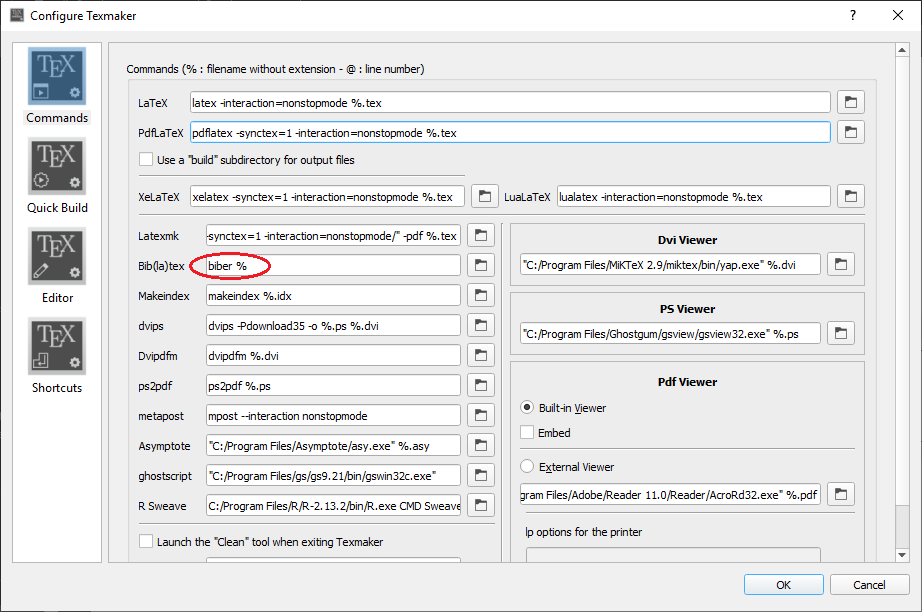
\includegraphics[width=.95\textwidth]{Intro_TexMakerConf.png}
    \caption[Screenshot of the main configuration settings in TexMaker.]{Screenshot of the main configuration settings in TexMaker.}
    \label{fig:Intro_TexMakerConf}    
\end{figure}
%%%%%%%%%%%%%%%%%%

	\item SVG images can be easily implemented although the explanation of how to install such a feature is still pending.
	\item TIF images can be easily implemented although the explanation of how to install such a feature is still pending.

\end{enumerate}


\subsection{Windows - TexStudio - MikTex}
Coming soon!

\subsection{Linux}
Coming soon!

\section{How to Use \textit{ThesiX}}
\ThesiX{} have the following structure:

\begin{lstlisting}
\documentclass[a4paper,11pt,openright]{book}
%%-------------------------------------------------------------
\def\iscodiretor{0}
\def\isfamousquote{1}
\def\isdedication{1}
\newcommand{\ThankThesiX}{This document make use of the latex template \textit{ThesiX}, originally made by I. Lombardero and available at https://github.com/ilomdez/ThesiX.}

%%-------------------------------------------------------------
\newcommand{\thesisauthor}{Iv\'{a}n Lombardero Hern\'{a}ndez}
\newcommand{\authordegree}{Graduado en Ciencias F\'{i}sicas}
\newcommand{\university}{UNIVERSIDAD POLIT\'{E}CNICA DE MADRID}
\newcommand{\school}{ESCUELA T\'{E}CNICA SUPERIOR DE INGENIEROS DE TELECOMUNICACI\'{O}N}
\newcommand{\departament}{Departamento de Electrónica Física, Ingeniería Eléctrica y Física Aplicada}
\newcommand{\institute}{INSTITUTO DE ENERG\'{I}A SOLAR}
\newcommand{\thetitle}{ThesiX: latex template for high-quality document formatting with special emphasis on thesis manuscripts - V1.0}
\newcommand{\publicationyear}{\the\year}
\newcommand{\thesisdirector}{Director Name}
\newcommand{\thesisdirectortitle}{Director Degree}
\newcommand{\thesiscodirector}{CoDirector Name}
\newcommand{\thesiscodirectortitle}{CoDirector Degree}

\newcommand{\blankpage}{\clearpage\mbox{}\newpage}
\newcommand{\pdfauthor}{\thesisauthor}
%%-------------------------------------------------------------
\newlength{\currentparskip}
\newenvironment{chapter_resume}% environment name 
{%
  \vspace{1cm}  
  \centering
      
  \setlength{\currentparskip}{\parskip}% save the value
  \begin{minipage}{0.65\textwidth}\setlength{\parindent}{0.5cm}
  \begin{itshape}
}% 
{\end{itshape}\end{minipage}\vspace*{\fill}\newpage}% end code
%-------------------------------------------------------------
\newenvironment{project}[4]{
\begin{itemize}[align=left, leftmargin=10mm, labelsep=1mm, labelwidth=2mm, itemindent=0pt]
	%\setlength{\itemindent}{-0.3in}
 	\item[\textbf{Title:}] #1
 	\item[\textbf{P.I:}] #2
 	\item[\textbf{Funding:}] #3
 	\item[\textbf{Duration:}] #4
\end{itemize} 
}
{\vspace{.5cm}}

%---------------------------------------------------------------
\newlength{\thicktopline}
\setlength{\thicktopline}{0.1em}
\newlength{\thickbottomline}
\setlength{\thickbottomline}{0.1em}
\newlength{\tablerowheight}
\setlength{\tablerowheight}{-1em} % Definition of basic info or LaTeX environments
%%
\newcommand{\app}{Appendix}
\newcommand{\aumet}{AuGe/Ni/Au}
\newcommand{\cha}{Chapter}
\newcommand{\equ}{Equation}
\newcommand{\ies}{Solar Energy Institute}
\newcommand{\iiiv}{III\=/V}
\newcommand{\iv}{I\nobreakdash-V}
\newcommand{\InN}{GaInNAs}
\newcommand{\InNSb}{GaInNAsSb}
\newcommand{\fig}{Figure}
\newcommand{\macmsq}{mA/cm\textsuperscript{2}}
\newcommand{\NSb}{GaNAsSb}
\newcommand{\pdmet}{Pd/Ge/Ti/Pd/Al}
\newcommand{\phosphoric}{H\textsubscript{3}PO\textsubscript{4}:H\textsubscript{2}O\textsubscript{2}:H\textsubscript{2}O}
\newcommand{\nip}{\textit{n\=/i\=/p}}
\newcommand{\pn}{\textit{pn}}
\newcommand{\sect}{Section}
\newcommand{\sj}{single\=/junction}
\newcommand{\soa}{state\=/of\=/the\=/art}
\newcommand{\tab}{Table}
\newcommand{\ThesiX}{\textit{ThesiX}}
\newcommand{\TJ}{GaInP/Ga(In)As/Ge}
\newcommand{\unitsscr}{$\Omega$·cm\textsuperscript{2}}
\newcommand{\unitssr}{$\Omega$/$\square$}

\newcommand{\Msup}{\$^\{}
\newcommand{\Msupe}{\}\$}

 % Definition of useful word shortcuts
% Packages used in ThesiX
%%-----------------------------------------------------------
% Embebing Fonts
% ¿Automatic in TexMaker? If you are using TeXStudio in Windows, Go to Options-> Configure TeXstudio->Commands->Ps2Pdf. In that field, just paste ps2pdf.exe -dPDFSETTINGS#/prepress -dEmbedAllFonts#true -dMaxSubsetPct#100 -dCompatibilityLevel#1.3 %.ps


%%-----------------------------------------------------------
% Debuging
%\usepackage{showframe}
%\usepackage{blindtext}
%\listfiles


%%------------------------------------------------------------
% Metadata
\usepackage[pdftex,hidelinks]{hyperref}
\hypersetup{pdftitle=\thetitle{}, pdfauthor={\thesisauthor}}
\hypersetup{pdfsubject={ThesiX LaTeX Template}}
\hypersetup{pdfkeywords={LaTeX, Thesis, Template, ILH}}


%%-----------------------------------------------------------
% General packages about encoding and appeareance
\usepackage[utf8]{inputenc}
\usepackage[top=1.75cm,bottom=1.75cm,left=2.5cm,right=2.5cm,includeheadfoot,asymmetric]{geometry}
\usepackage{newunicodechar}
\newunicodechar{µ}{\ensuremath{\mu}}
\newunicodechar{°}{º}
%\newunicodechar{α}{\ensuremath{\alpha}} %Esto se puede utilizar para caracteres chungos si va mal junto con el newunicodechar - fontec y inputtec de arriba , para los % quizas--
\usepackage{eurosym}
\usepackage{indentfirst}
\usepackage{enumitem}
\usepackage{amsmath}
\usepackage{amssymb} %Careful with the font loaded!! If it has already loaded the symmbols it may stop working
\usepackage{multirow}
%\usepackage{multicol}
\usepackage[shortcuts]{extdash} % unbreakable hyphen - dash
%\usepackage{xparse} %newcommand and newenvironment with multiple optional arguments
\usepackage{verbatim}
\usepackage{listings}
\lstset{
  basicstyle=\ttfamily,
  columns=fullflexible,
  frame=single,
  breaklines=true
}
\usepackage{pdfpages}


%%------------------------------------------------------------
% Titles, chapters, headers, etc.
\usepackage{fancyhdr}
\usepackage{titlesec}
\titleformat{name=\chapter,numberless}
	{\filcenter\normalfont\huge\bfseries}{}{20pt}{\Huge}[\vspace{0.0ex}\titlerule]
%
\titleformat{name=\chapter}[display]
	{\Huge\rm\filcenter}
	{\titlerule[2pt]%
	\vspace{-3pt}%
	\titlerule
	\vspace{1pc}%
	\Huge\rm\bfseries\MakeUppercase{\chaptertitlename} \Huge\rm\bfseries\MakeUppercase{\thechapter}}
	{1pc}
	{\titlerule
	\vspace{1pc}%
	\Huge}
%
\titleformat*{\subsubsection}{\large\itshape} % Definition of subsubsection style
\setcounter{secnumdepth}{3} % Depth of sections numbering - 3 =subsubsections
\setcounter{tocdepth}{2} %Depth of table of content - 2 =subsections


%%------------------------------------------------------------
% REFERENCES & GLOSSARIES
\usepackage{bookmark} % allows to set bookmarks manually, useful for abstract etc
\usepackage{cleveref} % for subfigures references and more
\usepackage{nameref}  % to reference section names
\newcommand{\itnameref}[1]{\textit{\nameref{#1}}} % reference section name in italics
\newcommand{\quitnameref}[1]{``\textit{\nameref{#1}}''} % reference section name in italics and quotation mars
\usepackage{tocbibind}
\usepackage[toc, acronym, nopostdot, section=chapter, automake=immediate]{glossaries}  %sort=def hace que super no pueda separar por grupos de palabras
% sanitizesort=false hace que pase del \textit{•} y cosas de esas y organice directamente por lo que ve dentro aunque según he leido ralentiza bastante - guia page 15
\makeglossaries
\usepackage[style=alphabetic, backend=biber, sortcites=true, sorting=ynt, defernumbers=true, maxbibnames=99]{biblatex}
\addbibresource{./bibliography/ThesisRef.bib}
%\assignrefcontextentries[]{*}
%\usepackage[hyphenbreaks]{breakurl}
%\usepackage{csquotes}
%
\DefineBibliographyStrings{english}{%
  bibliography={References},
}
\defbibheading{secbib}[\bibname]{%
  \section*{#1}%
  \markboth{#1}{#1}
}
%
\defbibenvironment{bibliographyNUM}
  {\list
     {\printtext[labelnumberwidth]{%
        \printfield{prefixnumber}%
        \printfield{labelnumber}}}
     {\setlength{\labelwidth}{\labelnumberwidth}%
      \setlength{\leftmargin}{\labelwidth}%
      \setlength{\labelsep}{\biblabelsep}%
      \addtolength{\leftmargin}{\labelsep}%
      \setlength{\itemsep}{\bibitemsep}%
      \setlength{\parsep}{\bibparsep}}%
      \renewcommand*{\makelabel}[1]{\hss##1}}
  {\endlist}
  {\item}


%%------------------------------------------------------------
% IMAGES
\usepackage{float} % Useful for tables as well
\usepackage{graphicx}
\usepackage{caption}
\usepackage{subcaption}
\captionsetup{labelfont=bf,justification=justified,font=footnotesize}
%\usepackage{wrapfig}
\graphicspath{
{./images/}
{./images/Title/}
{./images/Cover/}
{./images/Intro/}
}
\usepackage{svg}
%\setsvg{inkscape={C:/"Program Files"/Inkscape/inkscape.exe -z -D}}
%\usepackage[inkscapeexe=C:/Program~Files/Inkscape/inscape.exe]{svg}
\svgpath{{./images/}{./images/cover/}{./images/chapter1/}{./images/chapter2/}{./images/chapter3/}{./images/chapter4/}{./images/chapter5/}{./images/title/}}
%\def\eattif#1.tif{#1}
%\DeclareGraphicsRule{.tif}{png}{.png}{`convert #1 \eattif#1-tif-converted-to.png }
\usepackage{epstopdf}
\epstopdfDeclareGraphicsRule{.tif}{png}{.png}{convert #1 \OutputFile}
\AppendGraphicsExtensions{.tif}


%%-------------------------------------------------------------
% TABLES
\usepackage{tabularx}
\usepackage{makecell} %group words
\usepackage{booktabs}
\usepackage{array}
\usepackage{arydshln} % dash lines
\renewcommand\tabularxcolumn[1]{m{#1}}% for vertical centering text in X column - Not working always somehow
\newcolumntype{Y}{>{\centering\arraybackslash}X} % same as X but horizontally allinged
\newcolumntype{M}{>{\centering\let\newline\\\arraybackslash\hspace{0pt}}m{.5cm}}
%\newcolumntype{N}[1]{>{\centering\let\newline\\\arraybackslash\hspace{0pt}}Y}
\newcolumntype{n}{>{\centering\arraybackslash}m} % same as m but horizontally allinged
%%------------------------------------------------------------
% Force Words Htphenation
\hyphenation{
Ga-In-N-As-Sb
} % Packages and settings
% Acronym definitions
%
% A
\newglossaryentry{abc}{type=\acronymtype, name={ABC}, description={ABC example}}
\newglossaryentry{acronym1}{type=\acronymtype, name={AE1}, description={Acronym example 1}}
\newglossaryentry{acronym2}{type=\acronymtype, name={AE2}, description={Acronym example 2}}
%
% B
\newglossaryentry{b_acronym}{type=\acronymtype, name={BEA}, description={B example of acronym}}
%
% C
\newglossaryentry{c_acronym}{type=\acronymtype, name={CEA}, description={C example of acronym}}
%
%
% D
%
% E
%
% F
%
% G
%
% H
%
% I
%
% J
%
% K
%
% L
%
% M
%
% N
%
% O
%
% P
%
% Q
%
% R
%
% S
%
% T
%
% U
%
% V
%
% W
%
% X
%
% Y
%
% Z % Acronyms definition
% Symbols definitions
%
% A
\newglossaryentry{symbol1}{name={\textit{S\textsubscript{1}}}, description={Symbol example 1}}
\newglossaryentry{symbol2}{name={\textit{S\textsubscript{2}}}, description={Symbol example 2}}
\newglossaryentry{alpha_int}{name={$\alpha_int$}, description={Intrinsic Absorption coefficient}}
%
% B
\newglossaryentry{b_symbol}{name={B\textsuperscript{5}}, description={B example of symbol}}
%
% C
\newglossaryentry{c_symbol}{name={C\textsubscript{t}}, description={C example of symbol}}
%
%
% D
%
% E
%
% F
%
% G
%
% H
%
% I
%
% J
%
% K
%
% L
%
% M
%
% N
%
% O
%
% P
%
% Q
%
% R
%
% S
%
% T
%
% U
%
% V
%
% W
%
% X
%
% Y
%
% Z % Symbols definition
%-------------------------------------------------------
\begin{document}
\pagenumbering{gobble} %No page numbers
\begin{titlepage}
   \begin{center}
   		%\fontsize{17}{17}
   		%\selectfont
		\begin{LARGE}
		\textbf{\university}
		\end{LARGE}		   		
   		 		
   		\vspace*{2.5cm}
		
		\begin{normalsize}
		\school
 		\end{normalsize}
 		
 		\vspace*{1cm}
 		
 		
\includegraphics[scale=0.45]{LOGO_ESCUELA.pdf}

		\vspace{4.5cm}
		\vspace{\fill}

		\begin{Huge}
		\thetitle
		\end{Huge}
		
		\vspace{2.5cm}
		
		\begin{LARGE}
		\textbf{TESIS DOCTORAL} 
		\end{LARGE}
		
		
		\vspace{3cm}
		
		\begin{LARGE}
		\thesisauthor
		\end{LARGE}
		
		\begin{Large}
		\authordegree
		\end{Large}
		
		\vspace{1cm}
			
		\begin{LARGE}
		\publicationyear
		\end{LARGE}
   \end{center}
\end{titlepage}
\begin{titlepage}
   \begin{center}
   		%\fontsize{16}{16}\selectfont\textbf{\universidadupper}
		%\fontsize{16}{16}\selectfont
		\begin{LARGE}
		\textbf{\institute}
		\end{LARGE}
		
 		\begin{normalsize}
 		\departament
 		\end{normalsize}
		
		\vspace*{2.5cm}
		
		\begin{normalsize}
		\school
 		\end{normalsize}
% 		\begin{small}
%		\escuelaupper
% 		\end{small}		
		\vspace*{0.5cm}
 		
 		
\includegraphics[scale=0.4]{LOGO_ESCUELA.pdf}
		
		\vspace*{\fill}
		
		\begin{Huge}
		\thetitle
		\end{Huge}

		
		\vspace{2.5cm}
		
		\begin{table}[h]
		\LARGE
		\centering
		\begin{tabular}{l  l}
		
		\textbf{Autor:} & \thesisauthor \\
		 & \authordegree \\
		 & \\
		\if\iscodiretor0
		\textbf{Director:} & \thesisdirector \\
		\else
		\textbf{Directores:} & \thesisdirector \\
		\fi
		 				   & \thesisdirectortitle \\ 
						   \if\iscodiretor1						   
						   &  \thesiscodirector \\
						   & \thesiscodirectortitle \\
						   \fi
		\end{tabular}
		\label{tab:SecondTitle}
		\end{table}
				
		\vspace{1.5cm}
		
		\begin{LARGE}
		\publicationyear
		\end{LARGE}			
				
   \end{center}
\end{titlepage}
\newpage
\blankpage
\textbf{Tribunal nombrado por el Magfco. Y Excmo. Sr. Rector de la}

\textbf{Universidad Polit\'{e}cnica de Madrid.}

\vspace*{1cm}

PRESIDENTE:

\vspace*{1.5cm}

VOCALES:

%\indent\indent Guido es
%
%\indent\indent un poco retrasado
%
%\indent\indent y mi template es cojonudo
%{\setlength{\parindent}{0cm}
%\begin{table}[h]
%	\begin{tabular}{@{}ll}
%		VOCALES:	& Gerald Siefer \\
%					& Marta Vivar \\
%					& Eduardo Román Medina \\		
%	\end{tabular}
%\end{table}
\vspace*{3cm}

SECRETARIO:

\vspace*{1.5cm}

SUPLENTES:

\vspace*{3.5cm}

\hfill{Realizado el acto de defensa y lectura de la Tesis en Madrid,}

\hfill{el día \underline{\hspace{1cm}} de \underline{\hspace{2.5cm}} de 2019.}

\vspace*{1cm}

Calificaci\'{o}n:

\vspace*{2cm}

EL PRESIDENTE \quad\quad\quad\quad\quad\quad\quad\quad\quad\quad LOS VOCALES

\vspace*{2cm}

EL SECRETARIO
\blankpage
\vspace*{3.5cm}
\begin{flushright}
\textit{Dedication if any}
\end{flushright}
\newpage
\blankpage
\vspace*{3.5cm}
\begin{flushright}
\textit{Famous quote if any.\\Author}
\end{flushright}
\newpage
\blankpage
\pagestyle{fancy}
\fancyhf{}
%\renewcommand{\chaptermark}[1]{\markboth{#1}{}}
%\renewcommand{\sectionmark}[1]{\markright{\thesection\ #1}}
\fancyhead[CEO]{\itshape\nouppercase{\leftmark}}
\fancyfoot[C]{\thepage}
\setlength{\headheight}{15pt}

%\fancyhf{}
%\fancyhead[LE,RO]{\thepage}
%\fancyhead[LO]{\itshape\nouppercase{\rightmark}}
%\fancyhead[RE]{\itshape\nouppercase{\leftmark}}
\chapter*{Acknowledgements} \markboth{Acknowledgements}{}
Acknowledgements if any.
\frontmatter
\pdfbookmark[0]{Resumen}{Resumen}
\chapter*{Resumen} \markboth{Resumen}{}
Resumen means Abstract in Spanish, but obviously it should be replaced by the corresponding word in the mother tongue of the author. In my opinion, this should be always before the Abstract, as probably the acknowledgements will be mostly written in the author's mother tongue. Therefore it make sense to put these two sections together, and leave the Abstract closer to the rest of the document which will be probably written in English. In any case this depends on the personal view of the user.
\pdfbookmark[0]{Abstract}{Abstract}
\chapter*{Abstract} \markboth{Abstract}{}
Thesis abstract.
\tableofcontents
%\addcontentsline{toc}{chapter}{\listfigurename}
\listoffigures
%\addcontentsline{toc}{chapter}{\listtablename}
\listoftables
\setlength{\glsdescwidth}{0.7\textwidth}
\printglossary[type=main, style=super, nonumberlist, title=List of Symbols] %style=super, nogroupskip,
\setlength{\glsdescwidth}{0.8\textwidth}
\printglossary[type=\acronymtype, style=super, nonumberlist, title=List of Acronyms]
\mainmatter
\pagestyle{fancy}
\fancyhf{}
%\renewcommand{\chaptermark}[1]{\markboth{#1}{}}
%\renewcommand{\sectionmark}[1]{\markright{\thesection\ #1}}
%\fancyhead[R]{\textcolor{gray}{Mock Draft}}
\fancyhead[RO]{\rightmark}
\fancyhead[LE]{\leftmark}
\fancyfoot[RO,LE]{\thepage}
\setlength{\headheight}{15pt}
\renewcommand{\sectionmark}[1]{\markright{\thesection.\ #1}}
\renewcommand{\chaptermark}[1]{\markboth{\thechapter.\ #1}{}}
%\renewcommand{\chaptermark}[1]{\markleft{\thechapter.\ #1}}
%\fancyhead[RE]{\fontsize{10}{10}\selectfont\leftmark}
%\renewcommand{•}{•}
\chapter{Introduction}\label{ch:Intro}
\begin{chapter_resume}
This chapter presents the thesis introduction.\\

The current scenario of the photovoltaic market is briefly reviewed, analysing the historical trends and future perspectives of the most important technologies.\\

This leads to the revision of the \soa{} of multijunction solar cells, on which this thesis focuses on. The three main approaches (new compound materials, metamorphic buffers and the wafer bonding technique) are analysed, summarizing their benefits and drawbacks.\\

The aforementioned revision set the basis to establish the thesis goals, which is devoted to enhancing the potential of multijunction solar cells by developing advanced architectures. One of the main pathways has been the traditional approach based on increasing the number of subcells, but other improvements such as the thinning of substrates or the use of graphene as a top contact have also been explored. Accordingly, a detailed explanation of the main objectives to be accomplished is provided.\\

Afterwards, the outline followed in the thesis to illustrate the work carried out is explained to ease the reader task of finding whatever required information.\\

Finally, the framework which has surrounded this thesis is described, accounting for the funding, the means provided by the group, colleagues or third party partners as well as the main achievements attained through this thesis.\\
\end{chapter_resume}

\input{./chapters/Intro_sections/AboutThesiX}
\input{./chapters/Intro_sections/Installation}
\input{./chapters/Intro_sections/HowToUseThesiX}
\input{./chapters/Intro_sections/Outline}
\chapter{Elements}\label{ch:Elements}
\begin{chapter_resume}
This chapter contains examples of the main elements to be used in a document (figures, tables, references, etc.)

\vspace{0.7cm}

It has been written focusing on the user convenience, so that the code that makes every element is depicted so that it can be copied and paste to replicate it.
\vspace{0.7cm}

A more detailed explanation of the use of the code or the different possibilities will be explained in the chapters devoted to each element.
\end{chapter_resume}

\input{./chapters/Elements_sections/figures}
\input{./chapters/Elements_sections/tables}
\input{./chapters/Elements_sections/equations}
\input{./chapters/Elements_sections/crossrefs}
\input{./chapters/Elements_sections/lists}
%-----------------------------------------------------------------------
\pagestyle{fancy}
\fancyhf{}
%\renewcommand{\chaptermark}[1]{\markboth{#1}{}}
%\renewcommand{\sectionmark}[1]{\markright{\thesection\ #1}}
\fancyhead[CEO]{\itshape\nouppercase{\leftmark}}
\fancyfoot[C]{\thepage}
\setlength{\headheight}{15pt}

%\fancyhf{}
%\fancyhead[LE,RO]{\thepage}
%\fancyhead[LO]{\itshape\nouppercase{\rightmark}}
%\fancyhead[RE]{\itshape\nouppercase{\leftmark}}
\appendix
\input{appendix/appendix_Example}
%%----------------------------------------------------------------------
\chapter*{Bibliography}\markboth{Bibliography}{}
\addcontentsline{toc}{chapter}{Bibliography}
%\setbool{bbx:alpha}{true}
%\newrefcontext[sorting=nyt]
%\newrefcontext[sorting=nty]
%\raggedright
%\justify
\newrefcontext[sorting=nyt]
\printbibliography[heading=none] %secbib]
\endrefcontext
%[heading=bibintoc]
%
\chapter*{Publications}\label{ch:Publications}
%\newrefcontext[sorting=none,resetnumbers]
\markboth{Publications}{}
\addcontentsline{toc}{chapter}{Publications}
\begin{refsection}[./bibliography/Publications.bib]
\nocite{*}
%\setbool{bbx:alpha}{false}
\newrefcontext[sorting=ydnt]
\printbibliography[env=bibliographyNUM, heading=secbib, title=Journal Publications, type=article, resetnumbers=1]
\endrefcontext
\end{refsection}
\begin{refsection}[./bibliography/Publications.bib]
\nocite{*}
%\setbool{bbx:alpha}{false}
\newrefcontext[sorting=ydnt]
\printbibliography[env=bibliographyNUM, heading=secbib, title=Conference Publications, type=inproceedings]
\endrefcontext
\end{refsection}
\chapter*{Extra Information}\label{ch:ExtraInfo} \markboth{Extra Information}{}
\addcontentsline{toc}{chapter}{Extra Information}

Unnumbered chapter to add any relevant information that should not be part of the main chapters of the thesis itself nor an appendix. For instance, all the patents, awards, projects, etc. achieved or accomplished could be presented here, in one or different chapters. See the example below depicting the projects I was involved in during my thesis.

One last thing, although this chapter has been added after the bibliography, similar ones could be added at any place in the document with similar results. Nevertheless, attention should be paid to the page style, which might be set different depending on where the the chapter is placed in the \ThesiX{} template.\\

\begin{Large}
	\noindent\textbf{Projects as Principal Investigator}
\end{Large}

\begin{enumerate}[leftmargin=2.5mm, labelsep=-5mm]
	\setcounter{enumi}{0}
	%\setlength{\itemindent}{-2.5in}
	%\setlength{\itemindent}{-0.5in}	
	\item \begin{project}
	{Adelgazamiento de Células Solares para Reducir su Huella Ecológica y Maximizar su Rendimiento}
	{Iván Lombardero}
	{20,000\,\euro}
	{15/09/2019 - 15/09/2020}
	\end{project}
	
	\item \begin{project}
	{Desarrollo de Células Solares con Nitruros Diluidos de Última Generación para Alcanzar la Competitividad en la Energía Solar Fotovoltaica}
	{Iván Lombardero}
	{20,000\,\euro}
	{15/09/2018 - 15/09/2020}
	\end{project}
\end{enumerate}

\begin{Large}
	\noindent\textbf{Projects as Participant}
\end{Large}

\begin{enumerate}[leftmargin=2.5mm, labelsep=-5mm]
	\setcounter{enumi}{0}

\item \begin{project}
	{Evaluación de arquitecturas de nueva generación en células solares multiunión para lograr eficiencias del 50\,\%}
	{Carlos Algora}
	{314,358\,\euro}
	{01/01/2015 - 31/12/2017}
	\end{project}

\item \begin{project}
	{Dilute Nitride Based Concentrator Multijunction Solar Cells, With Efficiencies Over 47\,\%}
	{Carlos Algora}
	{191,250\,\euro}
	{11/12/15 - 30/11/18}
	\end{project}
\end{enumerate}
%%----------------------------------------------------------------------
\cleardoublepage  % Ensure finishing the last section on an even page
\pagestyle{empty} % Remove page number, headers, etc.
\blankpage        % Add two blankpages to add a final blank paper sheet
\blankpage
\end{document}
\end{lstlisting}

\section{Thesis outline} % Dar más detalles
This manual explains every step from the installation to the compilation of the \LaTeX{} template including the use of figures, lists, acronyms and many other useful elements to use in the course of any manuscript redaction. \ThesiX{} is outline as follows:
\begin{itemize}
	\item \cha\,\ref{ch:Intro}, \textit{\nameref{ch:Intro}}, reviews .
	\item Chapter 2 reviews .
	\item Chapter 3 analyses zed.
	\item Chapter 4  the simulations.
	\item Chapter 5 analysed.
	\item Chapter 6 summarizes work.
	\item Appendix A thesis.
	\item Appendix B gives .  
\end{itemize}
%\include{chapters/chapter_DN}
%\include{chapters/chapter_MJ}
%\include{chapters/chapter_Ge}
%\include{chapters/chapter_NewArch}
\chapter{Elements}\label{ch:Elements}
\begin{chapter_resume}
This chapter contains examples of the main elements to be used in a document (figures, tables, references, etc.)

\vspace{0.7cm}

It has been written focusing on the user convenience, so that the code that makes every element is depicted so that it can be copied and paste to replicate it.
\vspace{0.7cm}

A more detailed explanation of the use of the code or the different possibilities will be explained in the chapters devoted to each element.
\end{chapter_resume}

\section{Figures}\label{sec:Elements_figures}
%\begin{figure}[ht]
%\centering
%\includesvg[scale=0.5]{svgimage}
%\caption{A svg image example}
%\label{fig:x cubedvv graph}
%\end{figure}
\begin{lstlisting}
\begin{figure}[h]
\centering
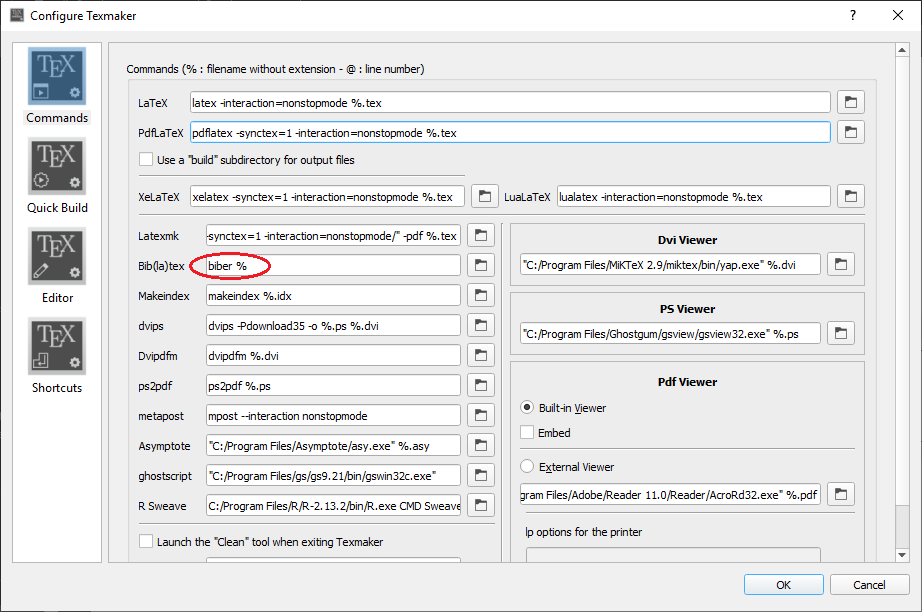
\includegraphics[width=.45\textwidth]{Intro_TexMakerConf.png}
\caption[Resume line]{An example graph}
\label{fig:example}
\end{figure}
\end{lstlisting}

\begin{figure}[h]
\centering
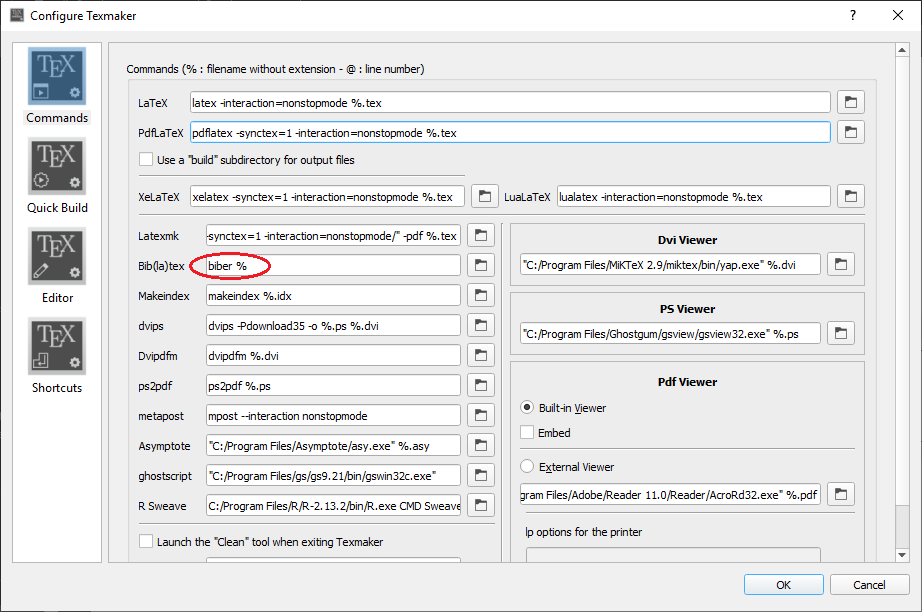
\includegraphics[width=.45\textwidth]{Intro_TexMakerConf.png}
\caption[Resume line]{An example graph}
\label{fig:example}
\end{figure}

\begin{lstlisting}
\begin{figure}[h]
    \centering
    \begin{subfigure}[b]{.3\textwidth}
        \centering
        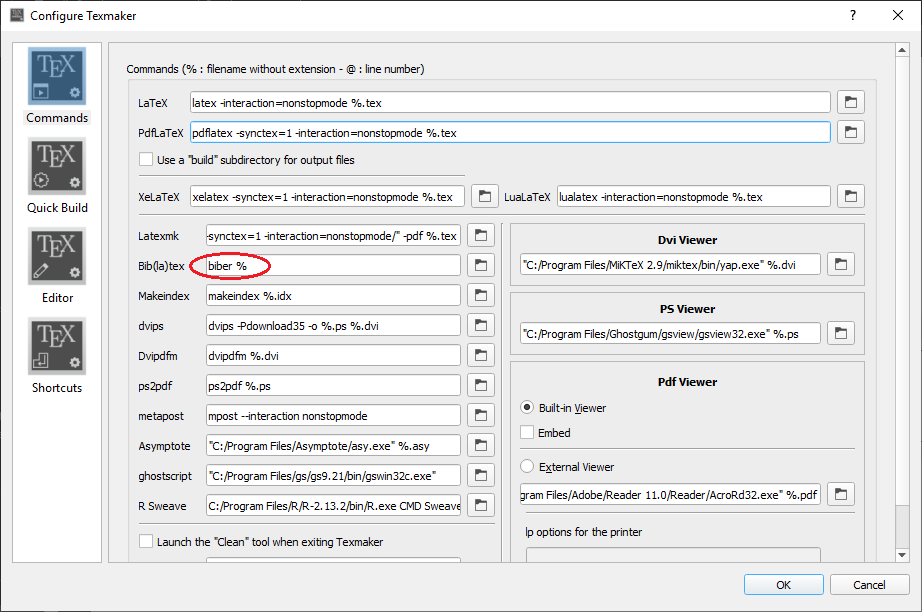
\includegraphics[width=\textwidth]{Intro_TexMakerConf.png}
        \caption{$y=x$}
        \label{fig:triple_x}
    \end{subfigure}
    \hfill
    \begin{subfigure}[b]{0.3\textwidth}
        \centering
        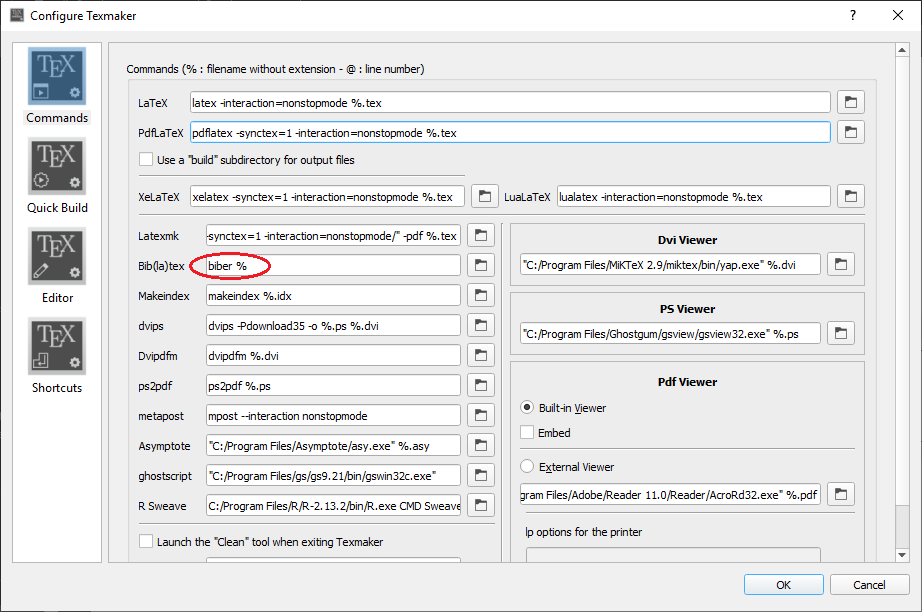
\includegraphics[width=\textwidth]{Intro_TexMakerConf.png}
        \caption{$y=3sinx$}
        \label{fig:triple_3sinx}
    \end{subfigure}
    \hfill
    \begin{subfigure}[b]{0.3\textwidth}
        \centering
        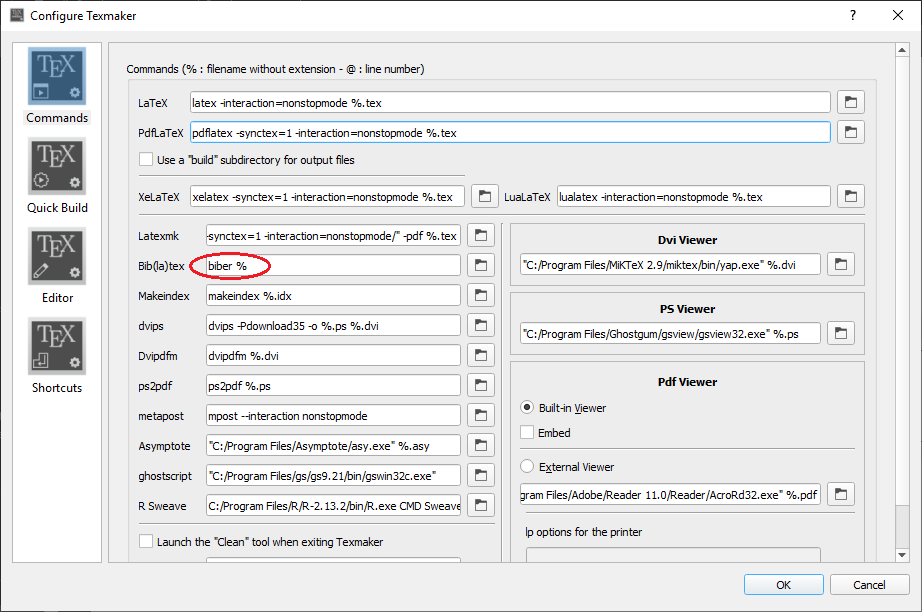
\includegraphics[width=\textwidth]{Intro_TexMakerConf.png}
        \caption{$y=5/x$}
        \label{fig:triple_5overx}
    \end{subfigure}
    \caption[Resume line]{Three simple graphs}
    \label{fig:triple}
\end{figure}
\end{lstlisting}

\begin{figure}[h]
    \centering
    \begin{subfigure}[b]{.3\textwidth}
        \centering
        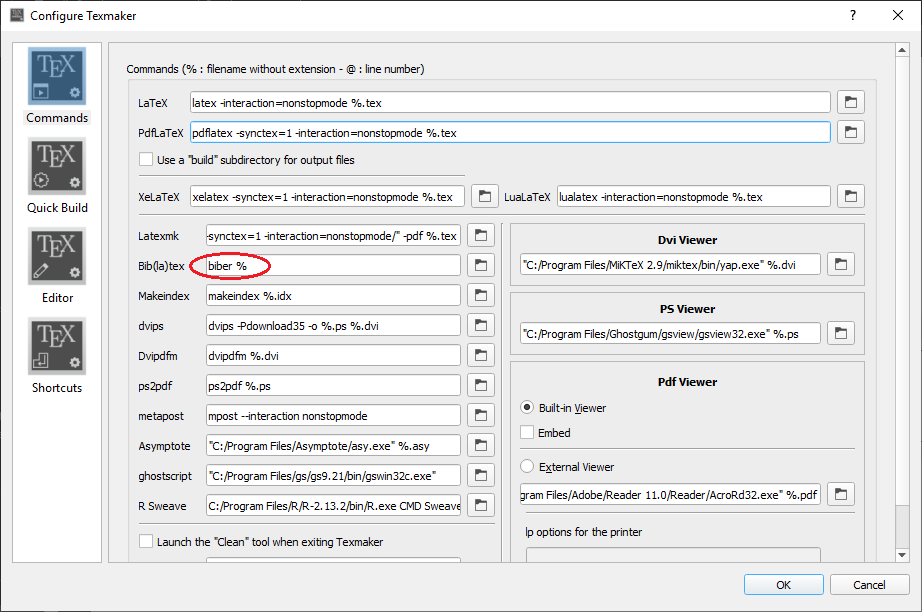
\includegraphics[width=\textwidth]{Intro_TexMakerConf.png}
        \caption{$y=x$}
        \label{fig:triple_x}
    \end{subfigure}
    \hfill
    \begin{subfigure}[b]{0.3\textwidth}
        \centering
        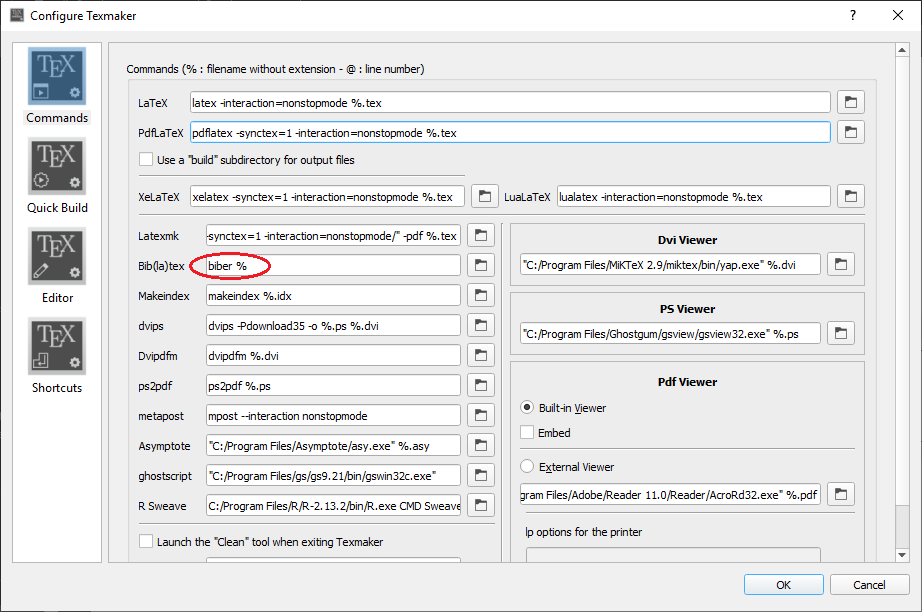
\includegraphics[width=\textwidth]{Intro_TexMakerConf.png}
        \caption{$y=3sinx$}
        \label{fig:triple_3sinx}
    \end{subfigure}
    \hfill
    \begin{subfigure}[b]{0.3\textwidth}
        \centering
        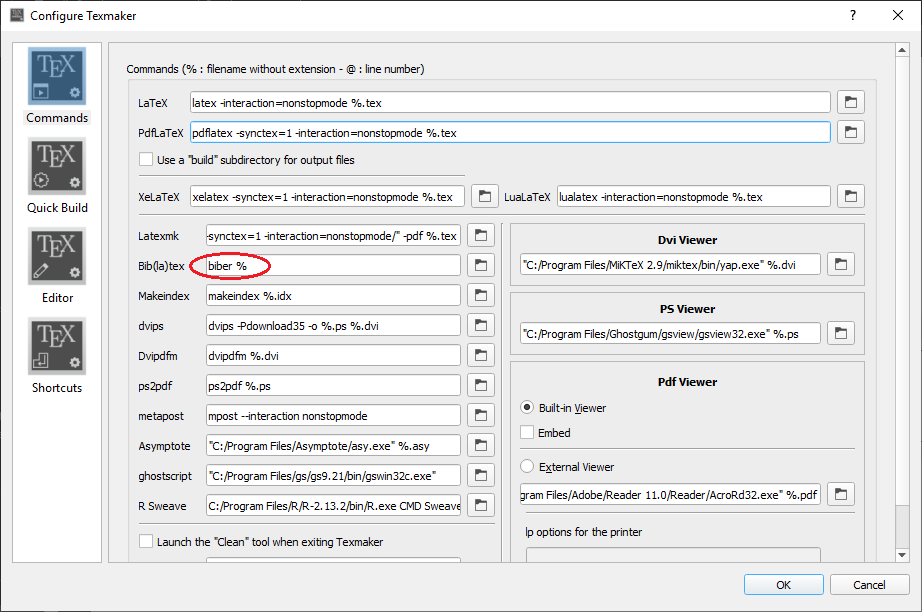
\includegraphics[width=\textwidth]{Intro_TexMakerConf.png}
        \caption{$y=5/x$}
        \label{fig:triple_5overx}
    \end{subfigure}
    \caption[Resume line]{Three simple graphs}
    \label{fig:triple}
\end{figure}
\section{Tables}\label{sec:Elements_tables}

\begin{lstlisting}
\begin{table}[ht]
	\centering
	\begin{tabular}{l | l | l}
	A & B & C \\
	\hline
	1 & 2 & 3 \\
	4 & 5 & 6
	\end{tabular}
	\caption{very basic table}
	\label{tab:example}
\end{table}
\end{lstlisting}

\begin{table}[ht]
	\centering
	\begin{tabular}{l | l | l}
	A & B & C \\
	\hline
	1 & 2 & 3 \\
	4 & 5 & 6
	\end{tabular}
	\caption{very basic table}
	\label{tab:example}
\end{table}
%
%\begin{table}[ht]
%    \begin{subtable}[h]{0.45\textwidth}
%        \centering
%        \begin{tabular}{l | l | l}
%        Day & Max Temp & Min Temp \\
%        \hline \hline
%        Mon & 20 & 13\\
%        Tue & 22 & 14\\
%        Wed & 23 & 12\\
%        Thurs & 25 & 13\\
%        Fri & 18 & 7\\
%        Sat & 15 & 13\\
%        Sun & 20 & 13
%        \end{tabular}
%        \caption{First Week}
%        \label{tab:week1}
%    \end{subtable}
%    \hfill
%    \begin{subtable}[h]{0.45\textwidth}
%        \centering
%        \begin{tabular}{l | c | c}
%        Day & Max Temp & Min Temp \\
%        \hline \hline
%        Mon & 17 & 11\\
%        Tue & 16 & 10\\
%        Wed & 14 & 8\\
%        Thurs & 12 & 5\\
%        Fri & 15 & 7\\
%        Sat & 16 & 12\\
%        Sun & 15 & 9
%        \end{tabular}
%        \caption{Second Week}
%        \label{tab:week2}
%    \end{subtable}
%    \caption{Max and min temps recorded in the first two weeks of July}
%    \label{tab:temps}
%\end{table}
\section{Equations}\label{sec:Elements_equations}
Ecuaciones:

\begin{enumerate}

\item In-line equation:

This is \lstinline"$E=mc^2$" in-line $\rightarrow$ This is $E=mc^2$ in-line

This is \lstinline"$\frac{\frac{1}{x}+\frac{1}{y}}{y-z}$" as well $\rightarrow$ This is $\frac{\frac{1}{x}+\frac{1}{y}}{y-z}$ as well\\

\item Numbered equation:

\begin{lstlisting}
\begin{equation}\label{eq:someequation}
\sqrt[n]{1+x+x^2+x^3+\dots+x^n}
\end{equation}
\end{lstlisting}

\begin{equation}\label{eq:someequation}
\sqrt[n]{1+x+x^2+x^3+\dots+x^n}
\end{equation}

\item Unnumbered equation:

\begin{lstlisting}
\begin{equation*}
\frac{n!}{k!(n-k)!} = \binom{n}{k}
\end{equation*}
\end{lstlisting}

\begin{equation*}
\frac{n!}{k!(n-k)!} = \binom{n}{k}
\end{equation*}
\end{enumerate}
\section{Cites}\label{sec:Elements_cites}
\begin{enumerate}
  \item Cita estándar:
  
  \verb=\cite{Hovel1997b}= $\rightarrow$  \cite{Hovel1997b}
  
  \verb=\cite{Rau2007,King2011}= $\rightarrow$  \cite{King2011,Rau2007}\\
  
  \item Cita comentada:
  
  \verb=\parencite[e.g.][page 300]{Miller2012}= $\rightarrow$ \parencite[e.g.][page 300]{Miller2012}
\end{enumerate}

\section{References}\label{sec:Elements_refs}

\begin{enumerate}
  \item Figure reference:
  
  \verb=\ref{fig:example}= $\rightarrow$ \ref{fig:example}
  
  \verb=\ref{fig:triple}= $\rightarrow$ \ref{fig:triple}\\
  
  \item Subfigure reference:
  
  \verb=\ref{fig:triple_x}= $\rightarrow$ \ref{fig:triple_x}
  
  \verb=\subref{fig:triple_x}= $\rightarrow$ \subref{fig:triple_x}\\
  
  \item Table reference:
  
  \verb=\ref{tab:example}= $\rightarrow$ \ref{tab:example}\\
  
  \item Equation reference:
  
  \verb=\ref{eq:someequation}= $\rightarrow$ \ref{eq:someequation}
  
  \verb=\eqref{eq:someequation}= $\rightarrow$ \eqref{eq:someequation}\\
  
  \item Chapter reference:
  
  \verb=\ref{ch:Elements}= $\rightarrow$ \ref{ch:Elements}
  
  \verb=\nameref{ch:Elements}= $\rightarrow$ \nameref{ch:Elements}\\
  
  \item Section reference:
  
  \verb=\ref{sec:Elements_refs}= $\rightarrow$ \ref{sec:Elements_refs}
  
  \verb=\nameref{sec:Elements_refs}= $\rightarrow$ \nameref{sec:Elements_refs}\\
\end{enumerate}


\section{Acronyms and symbols}\label{sec:Elements_acrosyms}
\begin{enumerate}
  \item Symbol:
  
  \verb=\gls{symbol1}= $\rightarrow$ \gls{symbol1}

  \item Acronym:

  \verb=\gls{acronym1}= $\rightarrow$ \gls{acronym1}
\end{enumerate}
\section{Lists}\label{sec:Elements_lists}
This is a list
\begin{lstlisting}
\begin{enumerate}
  \item First points
  \item Second
  \item Etc
\end{enumerate}
%\end{tabular}
Esto es una lista.
\end{lstlisting}

%\begin{tabular}{p{0.7\textwidth}}
\begin{enumerate}
  \item First points
  \item Second
  \item Etc
\end{enumerate}
%\end{tabular}

This is another list set to start at 8
  
\begin{lstlisting}
\begin{enumerate}
  \setcounter{enumi}{7}	
  \item First points
  \item Second
  \item Etc
\end{enumerate}
%\end{tabular}
Esto es una lista.
\end{lstlisting}

%\begin{tabular}{p{0.7\textwidth}}
\begin{enumerate}
  \setcounter{enumi}{7}
  \item First points
  \item Second
  \item Etc
\end{enumerate}
%\end{tabular}
\chapter{Statements}\label{ch:Statements}
\begin{chapter_resume}
Este capítulo contiene ejemplos sin explicacion de los distintos elementos que se pueden utilizar en esta plantilla de \LaTeX

\vspace{0.7cm}

La función de este capítulo no es explicar el uso ni el funcionamiento del código sino servir como referencia para poder copiar y pegar el código del elemento que se desee utilizar.
Es conveniente recordar que es útil tener un capítulo que incluya los principales elementos, ya que es útil para asegurar la correcta compilación de todos los paquetes. 
Es decir, incluye una referencia, un acrónimo y utiliza todos la mayoría de los paquetes por lo que nos permite chequear que el documento está correctamente diseñado.

\vspace{0.7cm}

Sin más, sólo recordar que para reproducir cualquier utilidad aquí mostrada no hay más que copiar el código fuente y pegarlo en el lugar deseado del documento.
\end{chapter_resume}
A continuación se muestran diferentes ejemplos para la inclusión de los principales elementos que se utilizarán a lo largo de la tesis: citas, acrónimos, símbolos, tablas, figuras y ecuaciones. Esta sección sólo incluye el código para incluir el elemento en cuestión, en el capítulo anterior se detalla cada elemento.
%\Blindtext

%\section{Tables}
%  \begin{enumerate}
%  \item Tabla:
%  
%  \textbackslash{}begin\{table\}[location]
% 
%  \textbackslash{}centering
%
%  \textbackslash{}begin\{tabular\}\{l \textbar{} c \textbar{} r\}
%
%  Label 1 \& Label 2 \& Label 3 \textbackslash{}\textbackslash{}
%
%  \textbackslash{}hline
%
%  1 \& 2 \& 3 \textbackslash{}\textbackslash{}
%
%  4 \& 5 \& 6 \textbackslash{}\textbackslash{}
%
%  7 \& 8 \& 9
%  
%  \textbackslash{}end\{tabular\}
%
%  \textbackslash{}caption\{Tabla simple\}
%
%  \textbackslash{}label\{tab:tablestatement\}
%
%  \textbackslash{}end\{table\}  
%
%  \begin{table}[ht]
%  \centering
%  \begin{tabular}{l | c | r}
%  Label 1 & Label 2 & Label 3 \\
%  \hline
%  1 & 2 & 3 \\
%  4 & 5 & 6 \\
%  7 & 8 & 9
%  \end{tabular}
%  \caption{Tabla simple}
%  \label{tab:tablestatement}
%  \end{table}
%\end{enumerate}
%\section{Figures}
%\begin{enumerate}
%  \item PNG/JPG/PDF:
%  
%  ``\textbackslash{}begin\{figure\}[location]
%  
%  \textbackslash{}centering
%  
%  \textbackslash{}includegraphics[options]\{Intro_TexMakerConf.png}
%
%  \textbackslash{}caption\{An example graph\}
%
%  \textbackslash{}label\{fig:x generalgraph\}
%
%  \textbackslash{}end\{figure\}''
%\begin{figure}[ht]
%\centering
%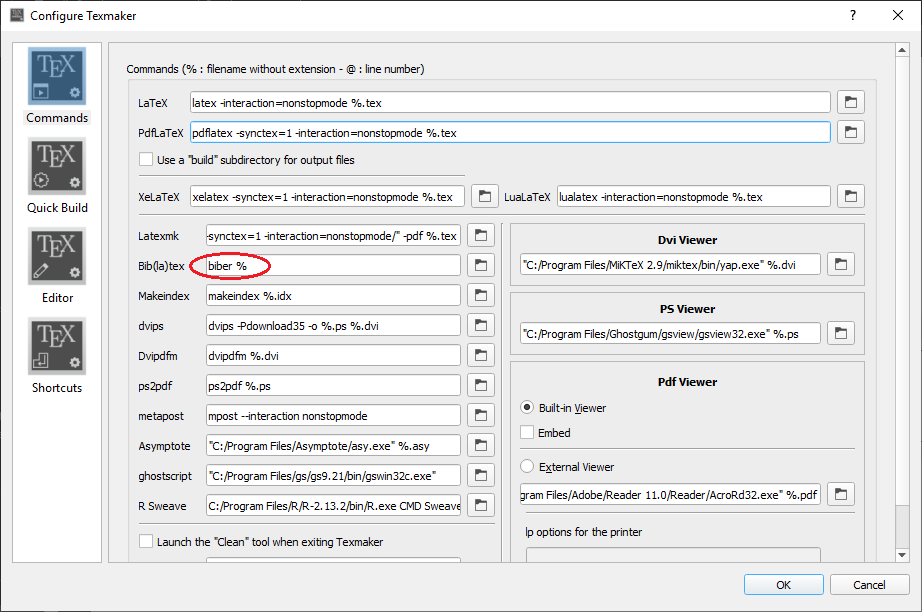
\includegraphics[scale=0.5]{Intro_TexMakerConf.png}
%\caption{PNG, JPG and PDF graph example}
%\label{fig:x generalgraph}
%\end{figure}
%  \item SVG:
%
%  ``\textbackslash{}begin\{figure\}[ht]
%  
%  \textbackslash{}centering
%
%  \textbackslash{}includesvg[options]\{svgimage\}
%
%  \textbackslash{}caption\{SVG graph statement example\}
%
%  \textbackslash{}label\{fig:x svgsatement\}
%
%  \textbackslash{}end\{figure\}''
%  \begin{figure}[ht]
%  \centering
%  \includesvg[scale=0.5]{svgimage}
%  \caption{SVG graph statement example}
%  \label{fig:x svgsatement}
%  \end{figure}
%\end{enumerate}
%\section{Lists}
%
%  \textbackslash{}begin\{enumerate\}
%  
%  \textbackslash{}setcounter\{enumi\}\{0\}
%
%  \textbackslash{}item Uno
%
%  \textbackslash{}item Dos
%
%  \textbackslash{}item Tres
%  
%  \textbackslash{}end\{enumerate\}
%
%\begin{enumerate}
%  \setcounter{enumi}{0}
%  \item Uno
%  \item Dos
%  \item Tres
%\end{enumerate}
%  
%  \textbackslash{}begin\{enumerate\}[font=\{\textbackslash{}color\{red!50!black\}\textbackslash{}bfseries\}]
%
%  \textbackslash{}setcounter\{enumi\}\{6\}
%
%  \textbackslash{}item Siete
%
%  \textbackslash{}item Ocho
%
%  \textbackslash{}item Nueve
%
%  \textbackslash{}end\{enumerate\}
%
%\begin{enumerate}[font={\color{red!50!black}\bfseries}]
%  \setcounter{enumi}{6}
%  \item Siete
%  \item Ocho
%  \item Nueve
%\end{enumerate}
%
%  \textbackslash{}begin\{itemize\}
%
%  \textbackslash{}item Item 1
%
%  \textbackslash{}item Item 2
%
%  \textbackslash{}item Item 3
%
%  \textbackslash{}end\{itemize\}
%  
%\begin{itemize}
%  \item Item 1
%  \item Item 2
%  \item Item 3
%\end{itemize}
%
%  \textbackslash{}begin\{enumerate\}[label=\{\textbackslash{}alph*\}]
%
%  \textbackslash{}item Item 1
%
%  \textbackslash{}item Item 2
%
%  \textbackslash{}item Item 3
%
%  \textbackslash{}end\{itemize\}
%  
%\begin{enumerate}[label={\alph*}]
%  %\setcounter{enumi}{6}
%  \item Item a
%  \item Item b
%  \item Item c
%\end{enumerate}
%
%  \textbackslash{}begin\{description\}
%
%  \textbackslash{}item [Volante] Controla la dirección de las ruedas
%
%  \textbackslash{}item [Acelerador] Controla la inyección de gasolina
%
%  \textbackslash{}item [Freno] Controla las pastillas de freno
%
%  \textbackslash{}end\{itemize\}
%  
%\begin{description}
%  \item [Volante] Controla la dirección de las ruedas
%  \item [Acelerador] Controla la inyección de gasolina
%  \item [Freno] Controla las pastillas de freno
%\end{description}
%

%\chapter{Ensure compilation chapter}\label{ch:Compilation}
\begin{chapter_resume}
This chapter puprpose is to ensure the correct compilation of the \LaTeX
\vspace{0.7cm}

Pues eso, al lío
\end{chapter_resume}


\section{One of each}
We are going to define at least on of each of all the possible elements in order to ensure that everything is working properly.


\subsection{Acronyms and symbols}
\gls{voc} and \gls{isc} are symbols
\gls{long} and \gls{eqe} are acronyms


\subsection{Figure}

\begin{figure}[ht]
\centering
\includegraphics[scale=0.5]{ace.png}
\caption{An example graph}
\label{fig:F0X_cubedgraph}
\end{figure}

\begin{figure}
    \centering
    \begin{subfigure}[b]{0.3\textwidth}
        \centering
        \includegraphics[width=\textwidth]{ace.png}
        \caption{$y=x$}
        \label{fig:F0X_threegraphs_A}
    \end{subfigure}
    \hfill
    \begin{subfigure}[b]{0.3\textwidth}
        \centering
        \includegraphics[width=\textwidth]{ace.png}
        \caption{$y=3sinx$}
        \label{fig:F0X_threegraphs_B}
    \end{subfigure}
    \hfill
    \begin{subfigure}[b]{0.3\textwidth}
        \centering
        \includegraphics[width=\textwidth]{ace.png}
        \caption{$y=5/x$}
        \label{fig:F0X_threegraphs_C}
    \end{subfigure}
    \caption{Three simple graphs}
    \label{fig:F0X_threegraphs}
\end{figure}

\begin{figure}[ht]
\centering
\includesvg[scale=0.5]{svgimage}
\caption{A svg image example}
\label{fig:F0X_svg}
\end{figure}



\subsection{Table}


\begin{table}[ht]
\centering
\begin{tabular}{l | l | l}
A & B & C \\
\hline
1 & 2 & 3 \\
4 & 5 & 6
\end{tabular}
\caption{very basic table}
\label{tab:T0X_abc}
\end{table}


\begin{table}[ht]
    \begin{subtable}[h]{0.45\textwidth}
        \centering
        \begin{tabular}{l | l | l}
        Day & Max Temp & Min Temp \\
        \hline \hline
        Mon & 20 & 13\\
        Tue & 22 & 14\\
        Wed & 23 & 12\\
        Thurs & 25 & 13\\
        Fri & 18 & 7\\
        Sat & 15 & 13\\
        Sun & 20 & 13
        \end{tabular}
        \caption{First Week}
        \label{tab:T0X_week1}
    \end{subtable}
    \hfill
    \begin{subtable}[h]{0.45\textwidth}
        \centering
        \begin{tabular}{l | c | c}
        Day & Max Temp & Min Temp \\
        \hline \hline
        Mon & 17 & 11\\
        Tue & 16 & 10\\
        Wed & 14 & 8\\
        Thurs & 12 & 5\\
        Fri & 15 & 7\\
        Sat & 16 & 12\\
        Sun & 15 & 9
        \end{tabular}
        \caption{Second Week}
        \label{tab:T0X_week2}
    \end{subtable}
    \caption{Max and min temps recorded in the first two weeks of July}
    \label{tab:T0X_week}
\end{table}
\subsection{cites and figure references}
Here are different cites \cite{Geisz2015} \ref{fig:F0X_cubedgraph} and \ref{ch:Compilation}
\ref{fig:F0X_threegraphs}
\ref{fig:F0X_threegraphs_A}
\ref{fig:F0X_threegraphs_B}
\ref{fig:F0X_threegraphs_C}
\ref{fig:F0X_svg}
\ref{tab:T0X_abc}
\ref{tab:T0X_week}
\ref{tab:T0X_week1}
\ref{tab:T0X_week2}

%-----------------------------------------------------------------------
\pagestyle{fancy}
\fancyhf{}
%\renewcommand{\chaptermark}[1]{\markboth{#1}{}}
%\renewcommand{\sectionmark}[1]{\markright{\thesection\ #1}}
\fancyhead[CEO]{\itshape\nouppercase{\leftmark}}
\fancyfoot[C]{\thepage}
\setlength{\headheight}{15pt}

%\fancyhf{}
%\fancyhead[LE,RO]{\thepage}
%\fancyhead[LO]{\itshape\nouppercase{\rightmark}}
%\fancyhead[RE]{\itshape\nouppercase{\leftmark}}
%%\include{chapters/future_works}
\appendix
%%\input{appendix/appendix_TCAD}
%%\input{appendix/appendix_Distributer}
%%\input{appendix/appendixC}
%%-----------------------------------------------------------------------
\chapter*{Bibliography}\markboth{Bibliography}{}
\addcontentsline{toc}{chapter}{Bibliography}
%\setbool{bbx:alpha}{true}
%\newrefcontext[sorting=nyt]
%\newrefcontext[sorting=nty]
%\raggedright
%\justify
\newrefcontext[sorting=nyt]
\printbibliography[heading=none] %secbib]
\endrefcontext
%[heading=bibintoc]
%
\chapter*{Publications}\label{ch:Publications}
%\newrefcontext[sorting=none,resetnumbers]
\markboth{Publications}{}
\addcontentsline{toc}{chapter}{Publications}
\begin{refsection}[./bibliography/Publications.bib]
\nocite{*}
%\setbool{bbx:alpha}{false}
\newrefcontext[sorting=ydnt]
\printbibliography[env=bibliographyNUM, heading=secbib, title=Journal Publications, type=article, resetnumbers=1]
\endrefcontext
\end{refsection}
\begin{refsection}[./bibliography/Publications.bib]
\nocite{*}
%\setbool{bbx:alpha}{false}
\newrefcontext[sorting=ydnt]
\printbibliography[env=bibliographyNUM, heading=secbib, title=Conference Publications, type=inproceedings]
\endrefcontext
\end{refsection}
%\chapter*{Projects}\label{ch:Projects} \markboth{Projects}{}
\addcontentsline{toc}{chapter}{Projects}
\begin{Large}
	\noindent\textbf{Projects as Principal Investigator}
\end{Large}

\begin{enumerate}[leftmargin=2.5mm, labelsep=-5mm]
	\setcounter{enumi}{0}
	%\setlength{\itemindent}{-2.5in}
	%\setlength{\itemindent}{-0.5in}	
	\item \begin{project}
	{Adelgazamiento de Células Solares para Reducir su Huella Ecológica y Maximizar su Rendimiento}
	{Iván Lombardero}
	{20,000\,\euro}
	{15/09/2019 - 15/09/2020}
	\end{project}
	\item \begin{project}
	{Desarrollo de Células Solares con Nitruros Diluidos de Última Generación para Alcanzar la Competitividad en la Energía Solar Fotovoltaica}
	{Iván Lombardero}
	{20,000\,\euro}
	{15/09/2018 - 15/09/2020}
	\end{project}
\end{enumerate}

\begin{Large}
	\noindent\textbf{Projects as Participant}
\end{Large}

\begin{enumerate}[leftmargin=2.5mm, labelsep=-5mm]
	\setcounter{enumi}{0}

\item \begin{project}
	{Evaluación de arquitecturas de nueva generación en células solares multiunión para lograr eficiencias del 50\,\%}
	{Carlos Algora}
	{314,358\,\euro}
	{01/01/2015 - 31/12/2017}c
	\end{project}

\item \begin{project}
	{Dilute Nitride Based Concentrator Multijunction Solar Cells, With Efficiencies Over 47\,\%}
	{Carlos Algora}
	{191,250\,\euro}
	{11/12/15 - 30/11/18}
	\end{project}
	
\item \begin{project}
	{Nitruros diluidos crecidos por \gls{movpe} con propiedades fotovoltaicas mejoradas para células solares multiunión de alta eficiencia}
	{Carlos Algora}
	{331,540\,\euro}
	{1/1/18 - 31/12/2020}
	\end{project}
	
\item \begin{project}
	{Desarrollo de Sistemas Fotovoltáicos de Baja Concentración con Células de Alta Eficiencia y Sistemas de Seguimiento a Un Eje: THESEUS}
	{Carlos Algora}
	{319,351\,\euro}
	{2014 - 2017}
	\end{project}

\item \begin{project}
	{A Low Cost, High Efficiency, Optoelectronic HCPV Module for 1000\gls{suns} Operation}
	{Ignacio Rey\=/Stolle}
	{143,000\,\euro}
	{1/4/2016 - 31/7/2019}
	\end{project}
\end{enumerate}
%\chapter*{Patents \& Awards}\label{ch:Patents_Awards}\markboth{Patents \& Awards}{}
\addcontentsline{toc}{chapter}{Patents \& Awards}

\begin{Large}
	\noindent\textbf{Patents}
\end{Large}

I have developed a new manufacturing process and proposed it to be patented. An \gls{itp} was asked to the \gls{oepm} in order to get a first evaluation of the potential of the idea to be patented. The results of this report have been analysed by the \gls{upm} patent partner UNGRIA, which has forecasted a high probability to get the idea patented by the \gls{oepm}. Accordingly, the patent application is currently at the writing stage and is expected to be submitted in February with me (I.\,Lombardero) as the principal investigator.\\\vspace{1cm}

\begin{Large}
	\noindent\textbf{Awards}
\end{Large}

The grants and awards granted during the Ph.D. studies are presented below:

\begin{enumerate}
	\item P.I. of two Iberdrola projects (see \sect\,\nameref{ch:Projects}).
	\item Finalist of the \gls{upm} Innovatech 2T Challenge 2019 edition to the best \gls{upm} technology proposal (winner to be announced December 19\textsuperscript{th}).
	\item Grant to attend a one\=/week course at \gls{icfo} facilities (\textit{\gls{icfo} Schools on the Frontiers of Light})
	\item \gls{fpu} and \gls{fpu}\=/\textit{Short internship} national grants to carry out the Ph.D. studies and the internship at the Okada's group of the \gls{rcast} (University of Tokyo).
	\item Reviewer of the journal \textit{Solar Energy Materials and Solar Cells} (Elsevier). Impact Factor: 6,019 in 2019.
\end{enumerate}
-----------------------------------------------------------------------
\blankpage
\end{document}
\end{lstlisting}
